
\section{欢迎来到 \textbf{OI Wiki}。}

\begin{figure}[htbp]
  \centering
  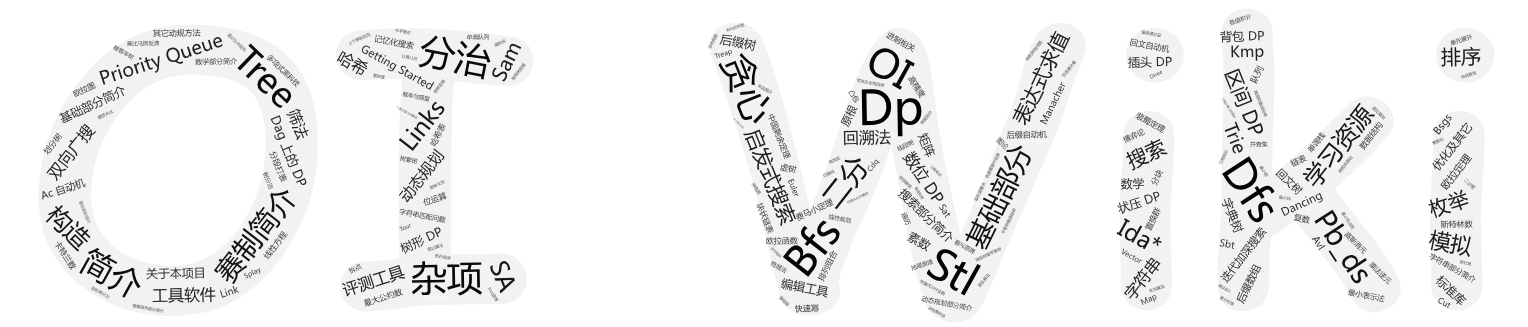
\includegraphics[width=0.7\textwidth]{docs/images/wordArt.png} 
  \caption{Word Art}
\end{figure}


\textbf{OI} (Olympiad in Informatics,信息学奥林匹克竞赛)在中国起源于 1984 年,是五大高中学科竞赛之一。自 1989 年起,每年还会选拔出国家集训队选手准备 IOI (International Olympiad in Informatics,国际信息学奥林匹克竞赛)。

\textbf{ICPC} (International Collegiate Programming Contest, 国际大学生程序设计竞赛)由 ICPC 基金会负责组织,是最具影响力的大学生计算机竞赛。ICPC 主要分为区域赛(Regional)和总决赛(World Finals)两部分。

\textbf{OI Wiki} 致力于成为一个免费开放且持续更新的知识整合站点,大家可以在这里获取关于 \textbf{编程竞赛 (competitive programming)} 有趣又实用的知识,我们为大家准备了竞赛中的基础知识、常见题型、解题思路以及常用工具等内容,帮助大家更快速深入地学习编程竞赛。

本项目受 \href{https://ctf-wiki.github.io/ctf-wiki/}{CTF Wiki} 的启发,在编写过程中参考了诸多资料,在此一并致谢。

本项目文档内容托管在 \href{https://github.com/24OI/OI-wiki}{GitHub},主要使用 \href{https://github.com/24OI/OI-wiki/issues}{Issues} / \href{https://jq.qq.com/?_wv=1027&k=5EfkM6K}{QQ} / \href{https://t.me/OIwiki}{Telegram} 进行交流沟通,期待你的加入。

Telegram 群组链接为 \href{https://t.me/OIwiki}{@OIwiki} , QQ 群号码为 \href{https://jq.qq.com/?_wv=1027&k=5EfkM6K}{588793226},欢迎加入。
